\chapter{Physically Based Rendering}

In order to generate photorealistic images, renderers must find accurate solutions to the \textit{rendering equation}. This chapter explains the meaning and intuition behind the equation, and describes how it can be solved by the path-tracing algorithm.

\section{The Rendering Equation}

The rendering equation describes the ``strength'' of light at each point in space and in each direction. To formalize the notion of strength, this section begins by introducing a few concepts from the study of radiometry.

\subsection{Radiometry}

In radiometry, there is a hierarchy of quantities that measure the strength of light in different contexts. The first quantity is \textit{radiant flux}, which measures the total energy that travels through a region of space per unit time in the form of electromagnetic radiation. Radiant flux is often denoted by $\Phi$, and its unit of measure is Watts($W$). 

In almost all regions in any scene, the radiant flux is not uniformly distributed, and thus one important quantity is the density of radiant flux with respect to area. This quantity is named \textit{irradiance}, which is denoted by $E$ and measured in power per unit area ($W\cdot m^{-2}$). Intuitively, irradiance measures the amount of light received by a single point in space. For this reason, in a region of space $S$, integrating the irradiance of each point in $S$ gives the total flux through $S$:
\begin{align}
    \Phi(S) = \int_S E(p) \d p 
    \label{irradiance integral}
\end{align}

For any point $p$, the irradiance $E(p)$ is not uniform across all directions, and thus it is also important to consider the density of irradiance in each direction $\omega$. This quantity, $L(p,\omega)$, is called \textit{radiance}, and it is measured in power per unit area per unit solid angle ($\text{W}\cdot\text{m}^{-2}\cdot \text{sr}^{-1}$). Radiance is an especially important quantity, because it is a measure of the strength of a single ray of light, identified by its direction $\omega$ and a point $p$ which it passes through. Consequently, radiance is the physical quantity that ray-tracing algorithms constantly operates in. 


In rendering, radiance often appears in the form $L_o(p,\omega)$ or $L_i(p,\omega)$, which denote the radiance going out of $p$ and those entering into it, respectively. More precisely, $L_o(p,\omega)$ represents the radiance that travels from $p$ and outwards in the direction $\omega$, and $L_i(p,\omega)$ represents the incoming radiance that travels towards to $p$ in the direction $-\omega$. The convention $L_i(p,\omega)$ might appear slightly counter-intuitive, since $\omega$ points in the opposite direction as the propagation of energy. However, the convenience of this notation will become apparent when the ray-tracing algorithm is formulated. 



\begin{figure}[H]
\centering
\tikzset{every picture/.style={line width=0.75pt}} %set default line width to 0.75pt        
\begin{tikzpicture}[x=0.75pt,y=0.75pt,yscale=-1,xscale=1]
%uncomment if require: \path (0,300); %set diagram left start at 0, and has height of 300

%Straight Lines [id:da6428603089338014] 
\draw    (70,220) -- (251,220) ;
\draw [shift={(160.5,220)}, rotate = 0] [color={rgb, 255:red, 0; green, 0; blue, 0 }  ][fill={rgb, 255:red, 0; green, 0; blue, 0 }  ][line width=0.75]      (0, 0) circle [x radius= 3.35, y radius= 3.35]   ;
%Straight Lines [id:da0998330538982608] 
\draw    (160.5,220) -- (218.58,162.41) ;
\draw [shift={(220,161)}, rotate = 495.24] [color={rgb, 255:red, 0; green, 0; blue, 0 }  ][line width=0.75]    (10.93,-3.29) .. controls (6.95,-1.4) and (3.31,-0.3) .. (0,0) .. controls (3.31,0.3) and (6.95,1.4) .. (10.93,3.29)   ;
%Straight Lines [id:da7334390340946089] 
\draw    (325,221) -- (506,221) ;
\draw [shift={(415.5,221)}, rotate = 0] [color={rgb, 255:red, 0; green, 0; blue, 0 }  ][fill={rgb, 255:red, 0; green, 0; blue, 0 }  ][line width=0.75]      (0, 0) circle [x radius= 3.35, y radius= 3.35]   ;
%Straight Lines [id:da024849495612862427] 
\draw    (480,160) -- (416.95,219.63) ;
\draw [shift={(415.5,221)}, rotate = 316.6] [color={rgb, 255:red, 0; green, 0; blue, 0 }  ][line width=0.75]    (10.93,-3.29) .. controls (6.95,-1.4) and (3.31,-0.3) .. (0,0) .. controls (3.31,0.3) and (6.95,1.4) .. (10.93,3.29)   ;
%Image [id:dp8436986937138125] 
\draw (161,245) node  {\includegraphics[width=27pt,height=30pt]{lightbulb.png}};
%Image [id:dp5859653893638117] 
\draw (498,154) node  {\includegraphics[width=27pt,height=30pt]{lightbulb.png}};

% Text Node
\draw (181,232) node [anchor=north west][inner sep=0.75pt]   [align=left] {$\displaystyle p$};
% Text Node
\draw (224,143) node [anchor=north west][inner sep=0.75pt]   [align=left] {$\displaystyle q$};
% Text Node
\draw (436,233) node [anchor=north west][inner sep=0.75pt]   [align=left] {$\displaystyle p$};
% Text Node
\draw (519,141) node [anchor=north west][inner sep=0.75pt]   [align=left] {$\displaystyle q$};


\end{tikzpicture}

\caption{Example: consider two points $p$, $q$, and $\omega=\frac{q-p}{|q-p|}$. On the left, the radiance sent from $p$ to $q$ is $L_o(p,\omega)$. On the right, the radiance received by $p$ from $q$ is $L_i(p,\omega)$.}
\end{figure}
Similar to equation \ref{irradiance integral}, which expresses flux as an integral of irradiance, it's also possible to obtain the incoming irradiance $E(p)$ by an integral across the incoming radiance from each direction. More precisely, the following relationship holds:
\begin{align}
    E(p) = \int_\Omega L_i(p,\omega_i)\cos\theta_i\d\omega_i
    \label{radiance integral}
\end{align}
Here, the support $\Omega$ is often a sphere or hemisphere of possible incoming directions, and the variable $\theta_i$ is the angle between $\omega_i$ and the surface normal. The cosine term accounts for the fact that for incoming rays that are not perfectly perpendicular to the surface, the differential area illuminated by the ray is multiplied by a factor $\frac{1}{\cos\theta_i}$, and thus the contribution per unit area should be multiplied by $\cos\theta_i$. 
\begin{figure}[H]
    \centering
  



    \tikzset{every picture/.style={line width=0.75pt}} %set default line width to 0.75pt        

    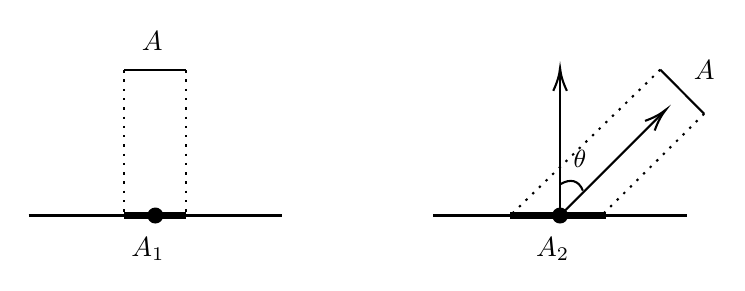
\begin{tikzpicture}[x=0.75pt,y=0.75pt,yscale=-1,xscale=1]
    %uncomment if require: \path (0,300); %set diagram left start at 0, and has height of 300
    
    %Straight Lines [id:da170514078900192] 
    \draw    (54,230) -- (176,230) ;
    \draw [shift={(115,230)}, rotate = 0] [color={rgb, 255:red, 0; green, 0; blue, 0 }  ][fill={rgb, 255:red, 0; green, 0; blue, 0 }  ][line width=0.75]      (0, 0) circle [x radius= 3.35, y radius= 3.35]   ;
    %Straight Lines [id:da016015541896946983] 
    \draw    (100,160) -- (130,160) ;
    %Straight Lines [id:da2875279917672757] 
    \draw  [dash pattern={on 0.84pt off 2.51pt}]  (100,160) -- (100,230) ;
    %Straight Lines [id:da4948721440011248] 
    \draw  [dash pattern={on 0.84pt off 2.51pt}]  (130,160) -- (130,230) ;
    %Straight Lines [id:da6791345652096885] 
    \draw [line width=2.25]    (100,230) -- (130,230) ;
    %Straight Lines [id:da17937256958328818] 
    \draw    (249,230) -- (371,230) ;
    \draw [shift={(310,230)}, rotate = 0] [color={rgb, 255:red, 0; green, 0; blue, 0 }  ][fill={rgb, 255:red, 0; green, 0; blue, 0 }  ][line width=0.75]      (0, 0) circle [x radius= 3.35, y radius= 3.35]   ;
    %Straight Lines [id:da5726229973180355] 
    \draw    (358.31,159.71) -- (379.42,181.02) ;
    %Straight Lines [id:da01972159484297009] 
    \draw  [dash pattern={on 0.84pt off 2.51pt}]  (358.31,159.71) -- (286,230) ;
    %Straight Lines [id:da8044979993297667] 
    \draw  [dash pattern={on 0.84pt off 2.51pt}]  (379.42,181.02) -- (329.69,230.29) ;
    %Straight Lines [id:da7389754977606782] 
    \draw [line width=2.25]    (286,230) -- (332,230) ;
    %Straight Lines [id:da7593939440598445] 
    \draw    (310,230) -- (310,161) ;
    \draw [shift={(310,159)}, rotate = 450] [color={rgb, 255:red, 0; green, 0; blue, 0 }  ][line width=0.75]    (10.93,-3.29) .. controls (6.95,-1.4) and (3.31,-0.3) .. (0,0) .. controls (3.31,0.3) and (6.95,1.4) .. (10.93,3.29)   ;
    %Straight Lines [id:da5048921054355329] 
    \draw    (310,230) -- (359.59,180.41) ;
    \draw [shift={(361,179)}, rotate = 495] [color={rgb, 255:red, 0; green, 0; blue, 0 }  ][line width=0.75]    (10.93,-3.29) .. controls (6.95,-1.4) and (3.31,-0.3) .. (0,0) .. controls (3.31,0.3) and (6.95,1.4) .. (10.93,3.29)   ;
    %Curve Lines [id:da665946044320908] 
    \draw    (310,215) .. controls (315,212) and (319,213) .. (321,218) ;
    
    % Text Node
    \draw (107,140) node [anchor=north west][inner sep=0.75pt]   [align=left] {$\displaystyle A$};
    % Text Node
    \draw (102,239) node [anchor=north west][inner sep=0.75pt]   [align=left] {$\displaystyle A_{1}$};
    % Text Node
    \draw (373,154) node [anchor=north west][inner sep=0.75pt]   [align=left] {$\displaystyle A$};
    % Text Node
    \draw (297,239) node [anchor=north west][inner sep=0.75pt]   [align=left] {$\displaystyle A_{2}$};
    % Text Node
    \draw (315,197) node [anchor=north west][inner sep=0.75pt]  [font=\small] [align=left] {$\displaystyle \theta $};
    
    
    \end{tikzpicture}
    

\caption{Example: on the right, the differential area $A_2$ illuminated by the ray is larger, because the ray is not perpendicular to the plane.}    
\end{figure}


\subsection{The BRDF}

In order to model the outgoing radiances at each point, it is essential to account for the fact that surfaces reflect incoming light. That is, for any direction $\omega_i$, the incoming radiance $L_i(p,\omega_i)$ may contribute to the outgoing radiance $L_o(p,\omega_o)$ of any other direction $\omega_o$. This relationship is captured by the bi-directional reflectance distribution function (BRDF), written as $f_r(p,\omega_o,\omega_i)$. Formally, the BRDF is defined as 
\begin{align}
    f_r(p,\omega_o,\omega_i) = \frac{\d L_o(p,\omega_o)}{\d E(p,\omega_i)}
    \label{BRDF def 1}
\end{align}
where $dE(p,\omega_i)$ represents the differential incoming irradiance at the direction $\omega_i$.

Using equation \ref{radiance integral}, it can be derived that 
\begin{align}
    dE(p,\omega_i) = L_i(p,\omega_i)\cos\theta_i\d\omega_i
\end{align}
which allows equation \ref{BRDF def 1} to be re-written as
\begin{align}
    f_r(p,\omega_o,\omega_i) = \frac{dL_o(p,\omega_o)}{L_i(p,\omega_i)\cos\theta_i\d\omega_i}
\end{align}
From this, it's straightforward to show that, for some $C$,
\begin{align}
    L_o(p,\omega_o) = \int_\Omega L_i(p,\omega_i)f_r(p,\omega_o,\omega_i)\cos\theta_i\d\omega_i + C
    \label{reflection plus C}
\end{align}

Different materials in the real world have drastically different BRDFs. The BRDF of a surface completely decides how it reflects light, which is a crucial factor of its appearances. This project implemented a range of different BRDFs corresponding to many different materials, but unfortunately, due to their complexity, details of these BRDFs could not be described here. 

~

In order to fully model $L_o(p,\omega_o)$, it remains to describe the term $C$ in equation \ref{reflection plus C}. Surfaces in the real world send outgoing radiances for two reasons only: they might emit light actively, and they reflect incoming light. Equation \ref{reflection plus C} already accounts for the reflected radiances, and thus it only remains to include actively emitted light. Writing $L_e(p,\omega_o)$ for the actively emitted radiance from $p$ towards the direction $\omega_o$, the following equation completely describes $L_o$:
\begin{align}
    L_o(p,\omega_o) = L_e(p,\omega_o) + \int_\Omega L_i(p,\omega_i)f_r(p,\omega_o,\omega_i)\cos\theta_i\d\omega_i
    \label{rendering equation}
\end{align}
This is the famous rendering equation, originally proposed by Kaijiya\cite{rendering_equation}. 


Under the assumption that radiance is constant along each ray, the incoming radiance $L_i(p,\omega_i)$ can be equated with the outgoing radiance from another point, $q$, as illustrated below.
\begin{figure}[H]
    \centering
    


\tikzset{every picture/.style={line width=0.75pt}} %set default line width to 0.75pt        

\begin{tikzpicture}[x=0.75pt,y=0.75pt,yscale=-1,xscale=1]
%uncomment if require: \path (0,300); %set diagram left start at 0, and has height of 300

%Straight Lines [id:da05220876887007719] 
\draw    (30,260) -- (211,260) ;
\draw [shift={(120.5,260)}, rotate = 0] [color={rgb, 255:red, 0; green, 0; blue, 0 }  ][fill={rgb, 255:red, 0; green, 0; blue, 0 }  ][line width=0.75]      (0, 0) circle [x radius= 3.35, y radius= 3.35]   ;
%Straight Lines [id:da8868681333199677] 
\draw    (150,230.5) -- (121.91,258.59) ;
\draw [shift={(120.5,260)}, rotate = 315] [color={rgb, 255:red, 0; green, 0; blue, 0 }  ][line width=0.75]    (10.93,-3.29) .. controls (6.95,-1.4) and (3.31,-0.3) .. (0,0) .. controls (3.31,0.3) and (6.95,1.4) .. (10.93,3.29)   ;
%Image [id:dp7926495246340768] 
\draw (232,169) node  {\includegraphics[width=27pt,height=30pt]{lightbulb.png}};
%Straight Lines [id:da34057240843922076] 
\draw  [dash pattern={on 0.84pt off 2.51pt}]  (150,230.5) -- (180,200) ;
%Straight Lines [id:da8846910740201797] 
\draw    (210,170) -- (181.41,198.59) ;
\draw [shift={(180,200)}, rotate = 315] [color={rgb, 255:red, 0; green, 0; blue, 0 }  ][line width=0.75]    (10.93,-3.29) .. controls (6.95,-1.4) and (3.31,-0.3) .. (0,0) .. controls (3.31,0.3) and (6.95,1.4) .. (10.93,3.29)   ;

% Text Node
\draw (141,272) node [anchor=north west][inner sep=0.75pt]   [align=left] {$\displaystyle p$};
% Text Node
\draw (255,155) node [anchor=north west][inner sep=0.75pt]   [align=left] {$\displaystyle q$};
% Text Node
\draw (123,163) node [anchor=north west][inner sep=0.75pt]   [align=left] {$\displaystyle L_{o}( q,-\omega _{i})$};
% Text Node
\draw (64,224) node [anchor=north west][inner sep=0.75pt]   [align=left] {$\displaystyle L_{i}( p,\omega _{i})$};


\end{tikzpicture}

\end{figure} 
Thus, defining the ray-tracing function $t(p,\omega_i)$ that computes the first surface point $q$ intersected by a ray originated from $p$ and travels in the direction $\omega_i$, the rendering equation is re-written as:
\begin{align}
    L_o(p,\omega_o) = L_e(p,\omega_o) + \int_\Omega L_o(t(p,\omega_i),-\omega_i)f_r(p,\omega_o,\omega_i)\cos\theta_i\d\omega_i
    \label{rendering equation with cast}
\end{align}

Finding solutions to this equation is the ultimate goal of rendering, because the job of any renderer is to compute the amount of radiance received by a hypothetical camera placed in the scene. For each point $p$ visible from the camera, the rendering algorithm must compute $L_o(p,\omega_o)$, where $\omega_o$ points from $p$ towards the camera. 

\section{Monte Carlo Integration}

Equation \ref{rendering equation with cast} cannot be solved analytically. Thus, rendering software solve the equation numerically using the method of Monte Carlo integration, and the algorithms used by these software are referred as ``integrators''. Given an integral
\begin{align*}
    I = \int_\Omega f(x) \d x,
\end{align*}
a Monte Carlo integrator randomly samples $N$ points $x_1,...,x_n\in \Omega$ according to some probability density function (PDF) $p$, and computes
\begin{align}
    I_N = \frac{1}{N}\sum_{i=1}^{N} \frac{f(x_i)}{p(x_i)}
    \label{monte carlo estimator}
\end{align}

It can be proved that this indicator is both unbiased $(E[I_N]=I)$ and consistent $(\lim_{N\to\infty}I_N = I)$. When applied to the rendering equation, the support $\Omega$ is the sphere or hemisphere of directions, and the function $f$ is computed by recursively estimating $L_o$, and then multiplying by the BRDF and the cosine of the direction.

\subsection{Importance Sampling}
\label{subsection IS}
In rendering, the variance $\Var[I_N]$ of the Monte Carlo estimator manifest in the form of random noise in the resulting image. Thus, variance reduction techniques are vital for rendering high-quantity images efficiently. One of the most important such techniques is importance sampling.

In the monte carlo estimator, the PDF $p$ used can be an arbitrary distribution. However, different distributions can lead to dramatically different variances. Importance sampling uses the fact that, informally, the variance $\Var[I_N]$ is reduced as the shape of the PDF $p(x)$ becomes similar to the shape of the integrand $f(x)$. As an example, consider when the PDF is 
$$ 
p(x)=\frac{f(x)}{\int_\Omega f(x') \d x'}.
$$ 
In this case, $p$ is always proportional to $f$, and the variance of the estimator is
\begin{align*}
\Var[I_N]
&= \frac{1}{N}\Var_{x\sim D}\left[\frac{f(x)}{p(x)}\right]\\
&= \frac{1}{N}\Var_{x\sim D}\left[\int_\Omega f(x') \d x'\right]\\
&=0
\end{align*}
It is of course infeasible to obtain a perfectly proportional PDF, because doing so requires computing the value of $\int_\Omega f(x') \d x'$, which is the value to be estimated in the first place. However, even if $p$ is similar in shape to $f$, variance can still be reduced.

\subsection{Multiple Importance Sampling}
\label{subsection MIS}
When solving the rendering equation, the integrand is the product of two factors: the incoming radiance $L_o(t(p,\omega_i),-\omega_i)$, and the reflectance $f_r(p,\omega_o,\omega_i)\cos\theta_i$. More generally, the renderer is solving an integration of the form
$$
I = \int_\Omega f(x)g(x)\d x
$$

In this case, if a renderer performs importance sampling according to distributions based on either $f$ or $g$, one of these two would often perform poorly\cite{pharr2016physically}. This is exactly the issue addressed by the technique of multiple importance sampling, or MIS.

MIS proposes that, during Monte Carlo Integration, samples should be drawn from multiple distributions, chosen in the hope that at least one will match the shape of the integrand well. MIS provides a way of weighting the samples from each distribution that eliminates large variance spikes due to mismatches between the integrand and the sampling density. More precisely, given a PDF $p_f$ that is a good match for $f$, and $p_g$ that is a good match for $g$, MIS draws $N$ samples $x_1,...,x_N$ from $p_f$, and $y_1,...,y_N$ from $p_g$, and apply the alternative Monte Carlo estimator:
\begin{align}
    I_N = \frac{1}{N} \sum_{i=1}^{N} \frac{f(x_i)g(x_i)w_f(x_i)}{p_f(x_i)} + \frac{f(y_i)g(y_i)w_g(y_i)}{p_g(y_i)}
    \label{MIS}
\end{align}
where the weights $w_f$ and $w_g$ are defined by
\begin{align*}
    w_s(x) = \frac{p_f(x)^2}{p_f(x)^2+p_g(x)^2}
\end{align*}
A full recount of why this weighting scheme reduces variance can be found in \cite{pharr2016physically}. 

To apply MIS when solving the rendering equation, the renderer samples from a PDF $p_{rad}$ that matches to the incoming radiance $L_o(t(p,\omega_i),-\omega_i)$, and another PDF $p_{ref}$ that matches the reflection term $f_r(p,\omega_o,\omega_i)\cos\theta_i$. In the path-tracer implemented in this project, $p_{rad}$ is a distribution that only samples $\omega_i$ that points to a light source, which is often much brighter than surfaces that indirectly reflects light. For $p_{ref}$, the project implemented specific sampling routings for each individual BRDF, thereby maximizing the similarity between the PDF and the BRDF at each point.


\section{The Path Space Formulation}
The rendering equation as written in equation \ref{rendering equation with cast} is inconvenient for deriving algorithms, because the relationship between geometries in the scene is implicit in the ray-tracing function $t(p,\omega_i)$. This section rewrites the equation into a from that makes this relationship more explicit.

Firstly, equation \ref{rendering equation with cast} is to be transformed from an integral over directions into an integral over area. Specifically, the variable of integration $\omega_i$, which represents an incoming direction, is to be replaced by a point $p_{src}$, which represents the source of the incoming ray. To achieve this, for any pair of mutually visible points $p,p'$, define 
\begin{align*}
    L_o(p'\to p) = L_o(p',\omega)\\
    L_e(p'\to p) = L_e(p',\omega)
\end{align*}
where $\omega = \frac{p-p'}{|p-p'|}$. Similarly, for three points $p,p',p''$, such that $p$ is visible from $p'$ and $p'$ is visible from $p''$, the BRDF at $p'$ is written as
\begin{align*}
    f_r(p''\to p'\to p) = f_r(p',\omega_o,\omega_i)
\end{align*} 
where $\omega_i = \frac{p''-p'}{|p''-p'|}$ and $\omega_o = \frac{p-p'}{|p-p'|}$.

Note that, since not all points $p_{src}$ is visible from $p$, the integrand needs to include a visibility term $V(p,p_{src})$, which takes the value 1 if $p_{src}$ is visible from $p$, and 0 otherwise. Furthermore, the change of variable also incurs a Jacobian term, which is $\frac{\cos\theta'}{|p-p_{src}|^2}$, with $\theta'$ being the angle between the incoming ray and the surface normal at $p_{src}$. Use these terms, equation \ref{rendering equation with cast} is rewritten so that for a ray from a point $p$ to the destination $p_{dest}$, the radiance is computed by
\begin{align*}
    L_o(p\to p_{dest}) =~ &L_e(p\to p_{dest}) \\
    &+ \int_A f_r(p_{src}\to p\to p_{dest}) L_o(p_{src}\to p)  V(p,p_{src}) \frac{cos\theta\cos\theta'}{|p-p_{src}|^2} \d p_{src}
\end{align*} 
where $A$ is the domain of all surface points in the scene. To simplify notation, write the term $G(p,p_{src})$ as $V(p,p_{src}) \frac{cos\theta\cos\theta'}{|p-p_{src}|^2}$, the equation becomes
\begin{align*}
    L_o(p\to p_{dest}) =~ &L_e(p\to p_{dest}) \\
    &+ \int_A f_r(p_{src}\to p\to p_{dest}) L_o(p_{src}\to p)  G(p,p_{src})  \d p_{src}
\end{align*} 

The equation above is referred to as the surface form light transport equation, and it can be interpreted as a recursive definition for $L_o$. Naturally, one can expand this recursive definition, and obtain an infinite sum:
\begin{align*}
    L_o(p_1\to p_0) =
    &L_e(p_1\to p_0)\\
    &+ \int_A L_e(p_2\to p_1)f_r(p_2\to p_1\to p_0)G(p_2,p_1) \d p_2\\
    &+ \int_A \int_A L_e(p_3\to p_2)f_r(p_3\to p_2\to p_1) G(p_3,p_2)f(p_2\to p_1\to p_0)G(p_2,p_1) \d p_3 \d p_2\\
    &+~...
\end{align*}
Here, each term represents the radiance contributed by paths of increasing length. For a path with $n$ reflection points, the source emission is $L_e(p_{n+1}\to p_{n})$, and it is weighted by a throughput term $T_n$, which is the product of the $f_r$ and $G$ at each reflection point:
\begin{align*}
    T_n = \prod_{i=1}^{n} f_r(p_{n+1}\to p_n\to p_{n-1})G(p_{n+1},p_n)
\end{align*}
Substituting this into the previous equation gives
\begin{align*}
    L_o(p_1\to p_0) = \sum_{n=0}^{\infty} \underbrace{\int_A \int_A...\int_A}_{n} L_e(p_{n+1}\to p_{n})T_n \d p_{n}\d p_{n-1}...\d p_1
\end{align*}


Notice that, the throughput term $T_n$ computes the portion of radiance that remains after $n$ reflections, which tends to decrease exponentially as $n$ increases. For this reason, it is natural to only consider the first few terms of this infinite sum (see figure \ref{fig maxdepth}). More precisely, given a maximum amount of reflections $MaxDepth$, the radiance $L_o(p_1\to p_0)$ can be estimated by 
\begin{align}
    L_o(p_1\to p_0) = \sum_{n=0}^{MaxDepth} \underbrace{\int_A \int_A...\int_A}_{n} L_e(p_{n+1}\to p_{n})T_n \d p_{n} \d p_{n-1}...\d p_1
    \label{rendering equation path tracing}
\end{align}

If a Monte Carlo estimator is used to approximate the integrals, the above formula becomes a recipe for a practical algorithm for computing radiances. This leads to the famous algorithm known as path-tracing, which is described in the next section.

\begin{figure}[H]
    \centering
    
    \begin{minipage}[t]{.45\textwidth}
        \centering
        \vspace{0pt}
        \includegraphics[width=.96\textwidth]{cornell_d1.png}
        \subcaption{$MaxDepth=1$}
    \end{minipage}
    \begin{minipage}[t]{.45\textwidth}
        \centering
        \vspace{0pt}
        \includegraphics[width=.96\textwidth]{cornell_d2.png}
        \subcaption{$MaxDepth=2$}
    \end{minipage}

    \vspace{0.3cm}

    \begin{minipage}[t]{.45\textwidth}
        \centering
        \vspace{0pt}
        \includegraphics[width=.96\textwidth]{cornell_d3.png}
        \subcaption{$MaxDepth=3$}
    \end{minipage}
    \begin{minipage}[t]{.45\textwidth}
        \centering
        \vspace{0pt}
        \includegraphics[width=.96\textwidth]{cornell_d4.png}
        \subcaption{$MaxDepth=4$}
    \end{minipage}
    \caption{Effect of increasing $MaxDepth$}
    \label{fig maxdepth}
\end{figure}

\section{The Path-Tracing Algorithm}

The path-tracing algorithm is parameterized by an integer, $spp$, which stands for samples per pixel. The algorithm samples $spp$ random points on each pixel to be rendered, and generate an initial ray corresponding to each sample point. Starting from the ray, the algorithm constructs $MaxDepth*2$ paths of increasing length, and accumulates the radiances carried by these paths. These radiances are combined by a MIS Monte Carlo estimator, which decides the final value of the pixel.

The path tracing integrator generates paths incrementally, starting from the camera location $p_0$. At each point $p_{n-1}$, the algorithm samples an incoming direction (for $p_{1}\to p_0$, the direction is fixed by the configuration of the camera), and traces the incoming ray to find $p_{n}$. If the point $p_{n}$ emits light actively, then this constitutes a path of $n-1$ reflection point. Moreover, $p_{n}$ also serves as the next reflection point, so the algorithm samples a point $p_{light}$ that illuminates $p_{n}$, and the radiance can be passed back to $p_0$ through a chain of reflections.


More precisely, the path tracing algorithm works as follows:


\begin{algorithm}[H]
    \label{Path Tracing}
    \SetKwProg{Fn}{Function}{:}{end}
    \ForEach{\upshape pixel in the image}{
        \For{\upshape $i$ from 1 to $spp$}{
            Generate the initial ray $r_0$ going out of the camera position $p_0$\;
            \For{\upshape $n$ from 1 to $MaxDepth$}{
                Find $p_n$ by computing the intersection between $r_{n-1}$ and the scene\;

                \If{\upshape $p_n$ is on a light source}{
                    Accumulate the radiance of the path $p_n\to p_{n-1}\to ... \to p_0$\;
                }
                
                Sample a point $p_{light}$ on a light source\;

                
                \If{\upshape the ray $p_{light}\to p_n$ is not occluded}{
                    Accumulate the radiance of the path $p_{light}\to p_n\to ... \to p_0$\;
                }
                
                Sample a direction $\omega_i$ from a PDF matching the BRDF at $p_n$\;

                Generate the ray $r_{n}$, originated at $p_n$ and points towards $\omega_i$\;
                
            }
            
        }
        Combine radiances computed by all samples to obtain final color of pixel\;
    }
    \caption{Path Tracing}
\end{algorithm}

~

Notice that, line 7 and 10 are two different ways a light emitter can illuminate $p_{n-1}$, and these two paths exactly correspond to the MIS procedure described in section \ref{subsection MIS}. When accumulating their radiances, the MIS weight should be applied.


For each pixel, the integrator estimates its color using a total of $spp*2*MaxDepth$ paths. Thus, as the parameter $spp$ increases, the variance of the Monte Carlo Estimator is reduced, which implies less noise in the rendered image. The following figure illustrates this effect.


\begin{figure}[H]
    \centering
    
    \begin{minipage}[t]{.45\textwidth}
        \centering
        \vspace{0pt}
        \includegraphics[width=.96\textwidth]{cornell_spp1.png}
        \subcaption{$spp=1$}
    \end{minipage}
    \begin{minipage}[t]{.45\textwidth}
        \centering
        \vspace{0pt}
        \includegraphics[width=.96\textwidth]{cornell_spp4.png}
        \subcaption{$spp=4$}
    \end{minipage}

    \vspace{0.3cm}

    \begin{minipage}[t]{.45\textwidth}
        \centering
        \vspace{0pt}
        \includegraphics[width=.96\textwidth]{cornell_spp16.png}
        \subcaption{$spp=16$}
    \end{minipage}
    \begin{minipage}[t]{.45\textwidth}
        \centering
        \vspace{0pt}
        \includegraphics[width=.96\textwidth]{cornell_spp64.png}
        \subcaption{$spp=64$}
    \end{minipage}
    \caption{Effect of increasing $spp$}
    \label{fig spp}
\end{figure}

For a typical scene, $spp$ is required to be at least 1024 in order to reduce noise down to an inconceivable level. Common images to be rendered consists of around 1 million pixels, thus around 1 billion pixel samples are often needed. Moreover, each ray generated in the algorithm needs to be tested for intersection with the entire scene, which often consists of millions of geometric primitives. The next chapter of this report will discuss how this project copes with this humongous amount of computation and implements an efficient path-tracing renderer.

